\documentclass{article}

% Language setting
% Replace `english' with e.g. `spanish' to change the document language
\usepackage[english]{babel}

% Set page size and margins
% Replace `letterpaper' with`a4paper' for UK/EU standard size
\usepackage[a4paper,top=2cm,bottom=2cm,left=3cm,right=3cm,marginparwidth=1.75cm]{geometry}

% Useful packages
\usepackage{amsmath}
\usepackage{fullpage}
\usepackage{amssymb}
\usepackage{amsthm}
\usepackage{bbm}
\usepackage{graphicx}
\usepackage{csquotes}
\usepackage[colorlinks=true, allcolors=blue]{hyperref}
\usepackage[style=alphabetic-verb]{biblatex}
\addbibresource{references.bib}
\usepackage{xcolor}
\newtheorem{definition}{Definition}
\newtheorem{theorem}{Theorem}[section]
\newtheorem{lemma}[theorem]{Lemma}
\newtheorem{corollary}[theorem]{Corollary}
\newtheorem{remark}[theorem]{Remark}

\newcommand\SB[1]{\textcolor{green}{#1}}









\title{Averaging on graphs: When does it work?}
\author{Martin Gjorgjevski}
\date{May 2022}
\DeclareMathOperator\supp{supp}
 \DeclareMathOperator{\LPM}{LPM}

\usepackage{microtype}

\begin{document}

\maketitle
\begin{abstract}
The content of this report is at the intersection of statistics and random graph theory.
Given a graph with a subset of labeled nodes, we are interested in the quality of the averaging estimator which for an unlabeled node predicts the average of the observations of its labeled neighbours. In order to describe the graph generating process we assume that nodes are associated to unobserved positions in $\mathbb{R}^d$ and that edges between nodes appear proportionally to the similarity of their associated positions as measured by a similarity kernel $k$. We rigorously study concentration properties, bias and variance bounds and
risk bounds under this assumption. While the estimator itself is very simple and the data generating process is too idealistic for practical applications, we believe that it is a useful playground for a theoretical understanding of quantities such as sample complexities and generalization bounds.
\end{abstract}



\tableofcontents




\section{Introduction}

\subsection{Regression on graphs}
\SB{I don't think this paragraph is about regression per se, it's about
  predicting graph signals}
Consider a social network (i.e. a graph) where people are represented as nodes
and relations between people are represented by edges, in which numerical data
of certain type is available only for some people in the network. How can the
missing data be estimated? For example, \textit{LinkedIn} is a social network
where people look for work and connections are often formed between people in
the same line of work.
\SB{It's not immediately clear in this example what the missing data is; I'd
  explain first what a ``graph signal'' is, that we expect them to be ``smooth''
over the graph as in your example, meaning that signal values don't differ too
much between neighbours, and finally that we can use this for prediction. This
gives you a natural way of introducing your estimator: average signal value over
neighbours.
Explain that this simple strategy hasn't really been studied. 
}
It is reasonable to expect that a candidate for a role should get the average of the salaries of his \textit{LinkedIn} connections. In reality the salary for a role depends on many factors such as level of education, previous work experience, geographical region and many other factors. However, it is reasonable to believe that connections formed on \textit{LinkedIn} have at least some similarities between these variables. In other words a candidate should not settle for a salary which is significantly lower than those of his coworkers, nor should he be able to get a salary which is significantly higher. This report is concerned with a theoretical analysis of  signal averaging on graphs which have latent 
geometric features.

\subsection{Averaging on graphs}
\SB{Not clear to the reader what exactly you're talking about here. What
  averaging? Are you talking about any technique that does prediction using some
  form of  smoothing? }
While it is intuitively clear that signal averaging on graphs in the context of
semi supervised learning \SB{SSL is sort of related but not the same thing} should work to at least some extent, it is important to acknowledge that such an attempt on estimation has firm limitations. It is by no means the state of the art method in the machine learning community. In fact, it is the simplest estimator in a graph regression context that one could think of. Nevertheless, signal averaging is used in many sophisticated algorithms such as Graph Neural Networks. T


To our knowledge there is no theoretical study on the limitations
\SB{performance, rather than limitations, you're not just studying limitations
}of this method in the machine learning literature. This is due to the lack of
statistical modeling in the graph structure \SB{Is it? How do you know?}. We
need to make assumptions about how such graphs are generated. In this report we
will adopt a popular framework for analyzing graph averaging known as the Latent
Position Model. With this goal in mind, we give some background on Random Graph
Models used in statistics.
\SB{The relevant distinction to make is between analyses that consider a fixed,
  given graph and look at the performance of a certain method for different
  classes of signals, and analyses that treat the graph as random. Point out
  that you are doing the latter, and have very weak assumptions on the signals.  }
\subsection{Random graphs}
\SB{You need a paragraph at the beginning of this section that defines random
  graphs, and explains which random graphs you are interested in and why}
\paragraph{The Erdos-Renyi Model}

The most well-known random graph model is the Erdos-Renyi random graph $G(n,p)$ with parameters $n\in\mathbb{N}$ and $0\leq p\leq 1$. This model samples a random graph on $n$ nodes with edges between nodes appearing independently with probability $p$. In other words, any two individuals have the same probability $p$ to form a connection, and connections between individuals are independent. This model is usually studied in the limit as $n\to\infty$ because of the concentration of measure phenomena. In their pioneering work Erdos and Renyi show that for many graphical properties such as connectedness or size of components a graph sampled from $G(n,p)$ has certain properties with overwhelming probability. In particular, there is a sharp threshold $p_c$ in the sense that for $p>p_c$ almost all $G(n,p)$ graphs have the property, while for $p<p_c$ almost none of them do. Classical examples are $p_c=1/n$ for the emergence of the giant component and $p_c=\log(n)/n$ for connectedness. 
\SB{Here would be a good place to point out that real world graphs do not have a
giant component}

\paragraph{Large Graphs from Real World Data}

Many large complex networks in the real world such as the World Wide Web, Movie
actor collaboration networks, Citation Networks to name a few, have properties
which are not present in the Erdos Renyi Random graph model. That is to say,
connections are not generated independently with equal probability. \SB{The
  previous two sentences are not equivalent, you can't link them with ``that is
  to say''} When such networks were compared
to Erdos-Renyi Random graph with same number of nodes and same average degree,
it was observed that cliques in the Real World Networks form more often than in
their Erdos-Renyi have counterpart. Similarly, Real World Networks have degree
distributions which typically obey a power law, i.e. the proportion of vertices
which have degree $k$ is of the order $k^{-\alpha}$, while for their Erdos-Renyi
model counterpart the same statistic should resemble a Poisson distribution.
Such observations prompted the scientific community to consider different models
for the data generating process which can better explain these phenomena
(\cite{Albert}, Section 2). Among the vast literature on this topic, we focus
our attention on two examples: the Stochastic Block Model and the Random
Geometric Graph.

\paragraph{The Stochastic Block Model} The Stochastic Block Model was introduced by Holland and Leindhart (\cite{Holland1983StochasticBF}). It assumes that the nodes of the observed graph naturally belong to communities and that the probability of edge between two vertices depends only on their communities. The main tasks for the Stochastic block model framework is community detection i.e. clustering vertices within their communities.

\paragraph{The Random Geometric Graph} Another popular random graph model is the Geometric Random Graph, which is generated by sampling $n$ independent random variables $X_1,...,X_n\in\mathbb{R}^d$ and placing edges between nodes $i$ and $j$ if the sampled points $X_i$ and $X_j$ are sufficiently close, i.e. there is some $h>0$ such that $P(i\sim j)=I(||X_i-X_j||\leq h)$. The value $h$ controls how well connected the graph is, in the sense that smaller values of $h$ give rise to sparser graphs. It is common to study how the behavior of certain graph statistics (such as empirical degree distributions, empirical average degrees and  empirical subgraph counts) changes with respect to $h$. A classical treatment of this topic is the Monograph of Penrose (\cite{Penrose2003RandomGG})
.

\begin{figure}
    \centering
    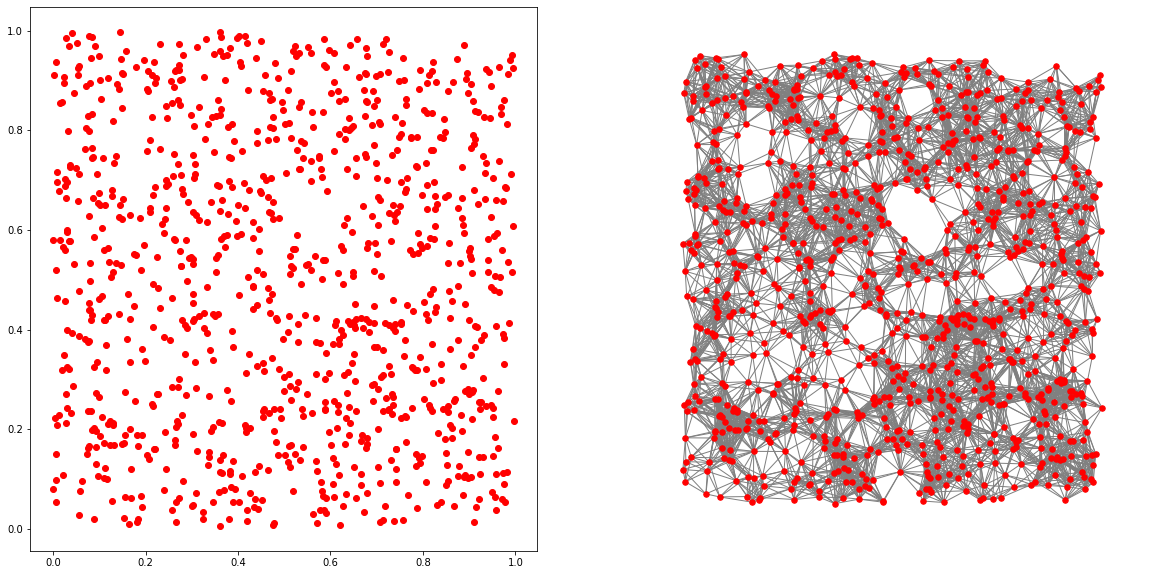
\includegraphics[width=1\textwidth]{sparse_rgg.png}
    \caption{Random Geometric Graph with $n=1000$ uniformly sampled points, $h=\sqrt{\frac{\log(n)}{n}}$}
    \label{Rgg_fig}
\end{figure}

\subsection{Latent Position Models}

The Latent Position Model (\cite{Hoff}) consists of three parameters:  the
number of nodes $n$, a similarity kernel on
$k\colon\mathbb{R}^d\times\mathbb{R}^d\to [0,1]$ and a probability density
function $p$ on $\mathbb{R}^d$. It generates a random graph on $n$ nodes in two
stages. First, a sample of i.i.d. variables $(X_1,...,X_n)$ with density $p$ is
drawn. The variable $X_i$ is called the latent position of node $i$. Second, a
Bernoulli variable with parameter $k(X_i,X_j)$ determines if there is an edge
between nodes $i$ and $j$. Intuitively this means that we are more likely to
observe an edge between two nodes which have positions that are similar with
respect to $k$. Clearly the Random Geometric Graph is a special case of a Latent
Position Model \SB{explain}. A slightly less obvious fact is that the Stochastic Block Model is a special case of a Latent Position model too, with latent dimension $d=1$. We choose to work with the Latent Position Model of a random graph as a data generating process because it is sufficiently general to cover a wide range of random graphs models on one hand and it is simple enough for theoretical considerations on the other.  
\begin{figure}[h!]
    \centering
    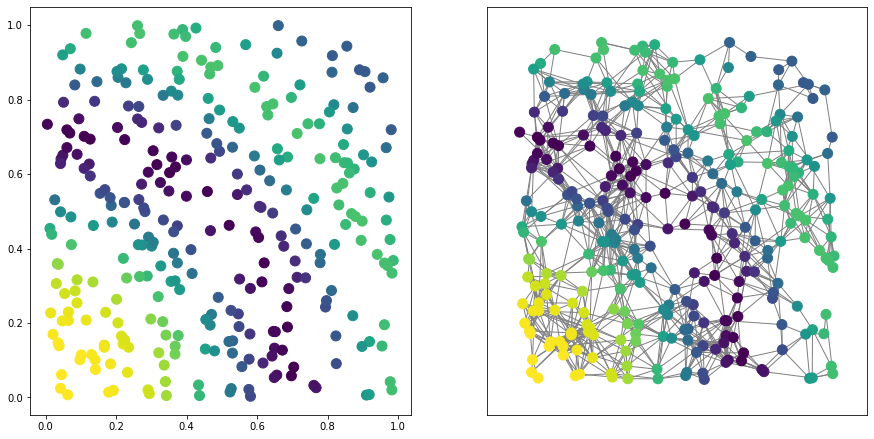
\includegraphics[width=1\textwidth]{lpm_image_correct.png}
    \caption{Latent position model with $n=300$ nodes, Gaussian kernel, and bandwith $h=0.75(\frac{\log(n)}{n})^{1/2}$}
    \label{fig:LPM_plot}
\end{figure}


\subsection{Nonparametric regression and the Nadaraya-Watson estimator}
Because of the kernel-based data-generating process in the Latent Position
Model, simple graph averaging is closely related to a popular weighted average
estimator known as the Nadaraya Watson estimator \SB{too abstract, expand and explain}. This observation motivates the name \textit{Graphical Nadaraya Watson} estimator. In the classical nonparametric regression problem  we are given data points $X_1,...,X_n\in[0,1]^d$ which are either fixed\footnote{For example equally spaced points on the unit cube $[0,1]^d$} or independent samples with common density $p$ and  
noisy observations $Y_i=f(X_i)+\epsilon_i$. Here, $f\colon [0,1]^d\to\mathbb{R}$ is an unknown function and in some suitable function class $\mathcal{F}$ and
$\epsilon_1,...,\epsilon_n$ are assumed to be i.i.d. centered variables with finite variance $\sigma^2$. The goal is to estimate $f$. The term \textit{nonparametric} stems from the fact that the function class $\mathcal{F}$ can not be parametrized by a subset of $\mathbb{R}^m$ for any $m\in \mathbb{N}$.
A basic idea for estimating $f$ at a point $x\in[0,1]^d$ is to average the observations $Y_i$ for which $|X_i-x|$ is smaller than a certain threshold. More precisely, given $h>0$ an intuitive estimator for $f(x)$ is

\begin{equation*}
    \hat{f}_{h}(x)=\begin{cases}
    \frac{\sum_{i=1}^nY_iI(|x-X_i|\leq h)}{\sum_{i=1}^nI(|x-X_i|\leq h)} \quad &\text{if}\, \sum_{i=1}^n 
    I(|x-X_i|\leq h)>0\\
    0 \quad &\text{otherwise}\\
    \end{cases}
\end{equation*}
More generally one can consider weighted averages which depend on the distance in a more sensitive manner so that the weights  

This is a special case of the \textit{Nadaraya Watson} estimator:

\begin{equation}
\label{NW_def}
    \hat{f}_{NW,h}(x)=\begin{cases}
    \frac{\sum_{i=1}^nY_iK(\frac{x-X_i}{h})}{\sum_{i=1}^n{K(\frac{x-X_i}{h}})} \quad &\text{if}\, \sum_{i=1}^n 
    K(\frac{x-X_i}{h})\neq 0\\
    0 \quad &\text{otherwise}\\
    \end{cases}
\end{equation}
The parameter $h>0$ is called the bandwith. 

\begin{figure}
    \centering
    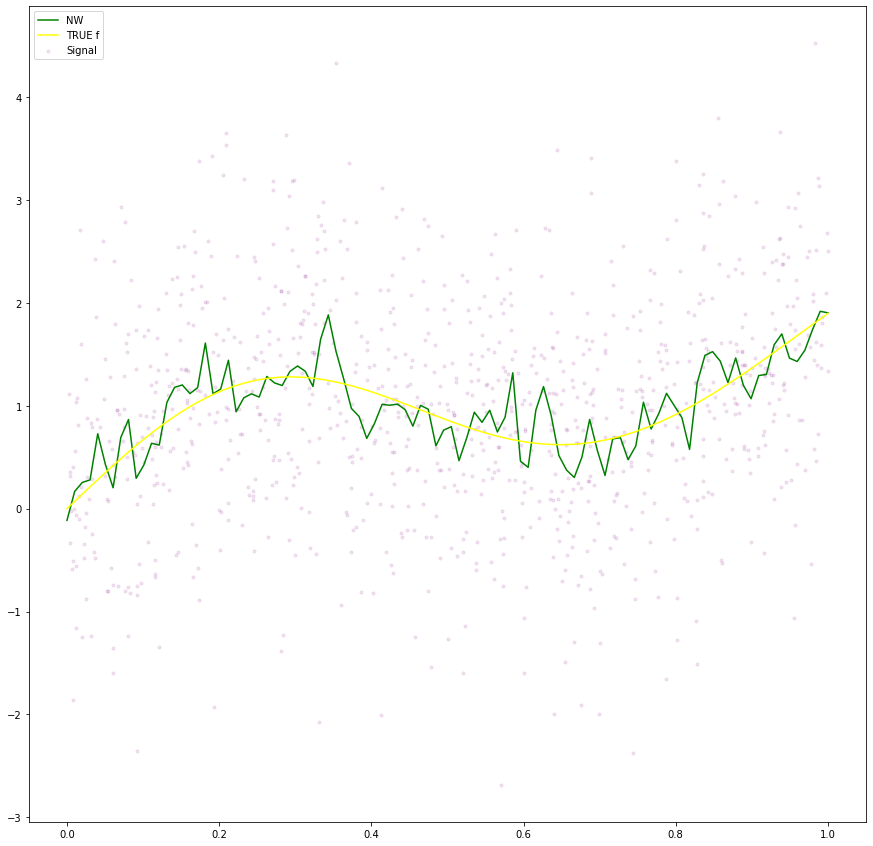
\includegraphics[width=0.45\textwidth]{low_bias_001.png}
    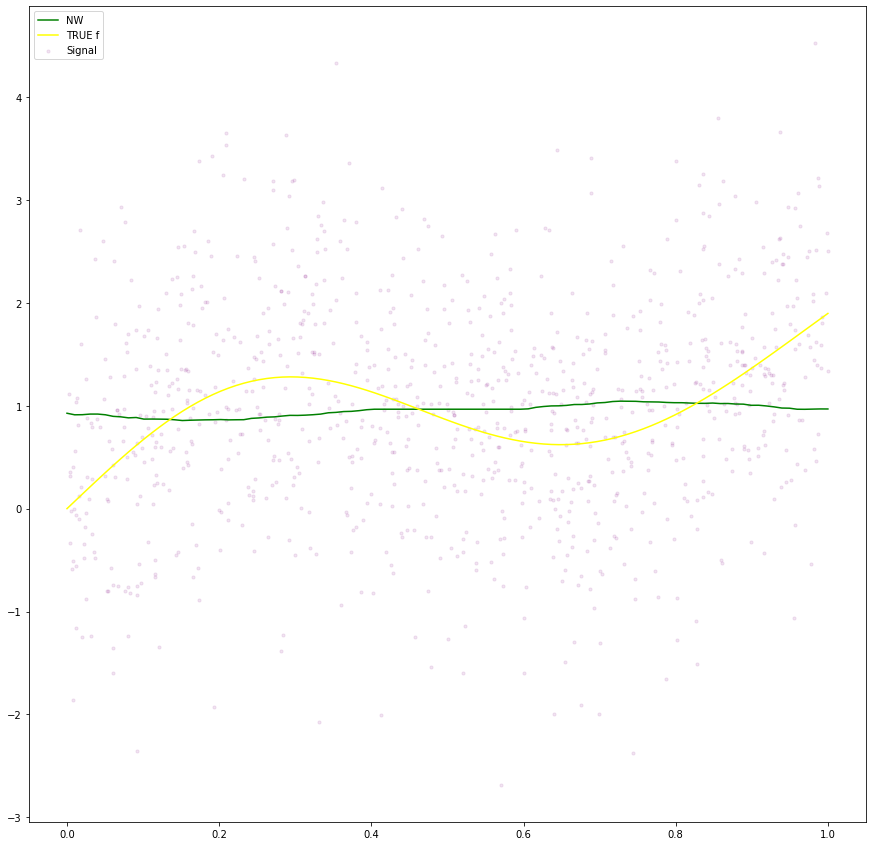
\includegraphics[width=0.45\textwidth]{low_variance_06.png}
    \caption{Bias-Variance Tradeoff: n=1000 points are sampled uniformly and
      independently on $[0,1]$ and gaussian noise with variance $\sigma^2=1$ is
      added. Left: $\hat{f}_{NW}$ estimator with $h=0.01$. Right: $\hat{f}_{NW}$
      estimator with $h=0.6$ $\hat{f}_{NW}$. \SB{Good illustration, but fonts
        are too small, axes are unlabeled, yellow curve is barely visible. Add a
      comment saying left panel is high-variance, low-bias and right panel is
      the opposite.}
 }
    \label{fig_nw_sensitivity}
\end{figure}

\begin{figure}
    \centering
    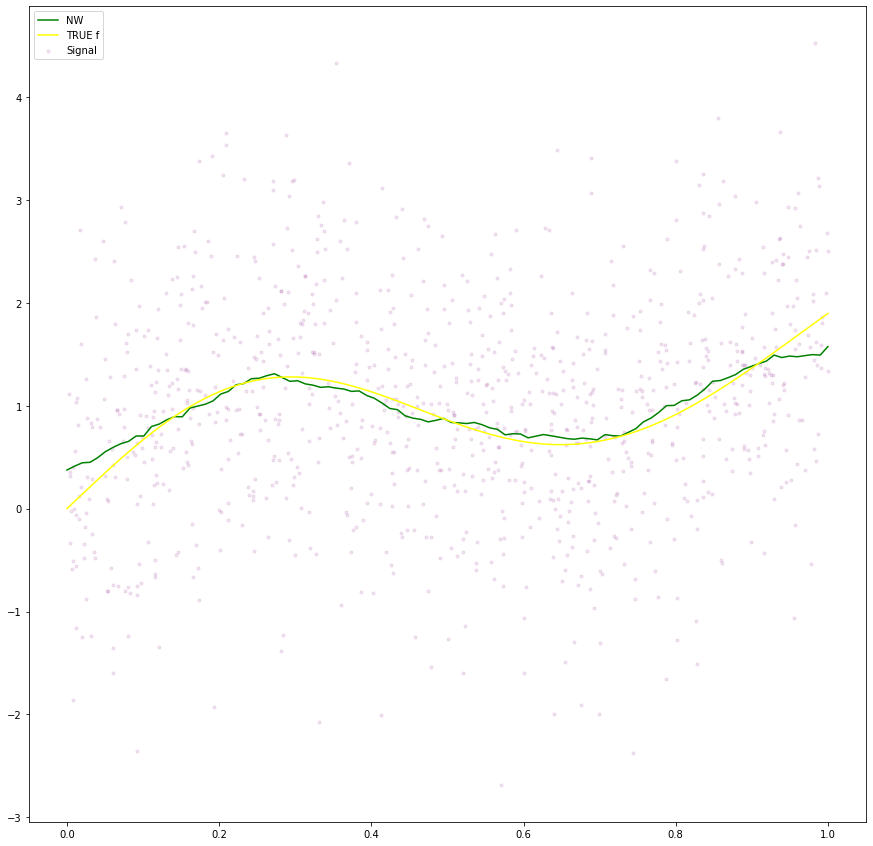
\includegraphics[width=0.45\textwidth]{bias_variance_tradeof_01.png}
    \caption{Same setting as figure \ref{fig_nw_sensitivity}, $\hat{f}_NW$ estimator with $h=0.1$}
    \label{fig_nw_bias_var_tradeoff}
\end{figure}


The quality of the estimator in terms of the $L^2$-risk
$E((\hat{f}_{NW}(x)-f(x))^2$ at a fixed point $x\in\mathbb{R}^d$ will depend on
the many factors, such as the regularity of $f$, the choice of the kernel $k$
but most importantly on the choice of bandwith $h>0$. The $L^2$-risk admits the so-called bias-variance decomposition

\begin{equation}
\label{eqn:bias-variance-decomp}
E(\hat{f}_{NW}(x)-f(x))^2=Var(\hat{f}_{NW}(x))+(E\hat{f}_{NW(x)}-f(x))^2
\end{equation}
The quantity $E(\hat{f}_{NW}(x)-f(x))$ is known as ``bias'' and under regularity assumptions on $f$ such as $\alpha$-Hölder continuity, this term is upper bounded by $Ch^{\alpha}$ where $C$ depends on $k$ and $\alpha$ but not on the sample size $n$. We will give a more thorough discussion of the bias in Chapter 4. On the other hand, the variance $Var(\hat{f}_{NW}(x)$ tends to increase as $h$ decreases, this is the famous bias-variance tradeoff phenomenon. In the fixed design setting optimal rates for $h$ are available, and they are dependent on the sample size $n$ (see \cite{Tsybakov} section 1.5 and section 1.6, Proposition 1.13). The main takeaway is that the statistician should adapt $h$ with respect to the sample size $n$. 


 \section{Framework}
\paragraph{Framework} We observe a random graph with vertex set $[n+1]$  sampled
according to an $\LPM(n+1,k_n,p)$ and assume that for nodes $i=1,...n$ (all but
the last node) there is a label \SB{observation, label is for classification
  problems exclusively} of the form $Y_i=f(X_i)+\epsilon_i$ with $f\colon\mathbb{R}^d\to\mathbb{R}$. Besides the graph itself and the explanatory variables $Y_1,...,Y_n$ no other quantities are assumed to be known. We write $X$ in place of $X_{n+1}$ and for $i=1,...,n$ we write $a(X,X_i)$ for the indicator that there is an edge between the node $n+1$ and node $i$. To describe edge generation more precisely, we assume that for $i=1,...,n$ the indicator of an edge between $X$ and $X_{i}$ is given by 

\begin{equation*}
    a(X,X_{i})=I(U_i\leq k(X,X_i))
\end{equation*}
where $U_1,...,U_n$ are uniform variables on $[0,1]$, such that $(U_1,...,U_n,X_1,...,X_n,X,\epsilon_1,....,\epsilon_n)$ are jointly independent variables. For $x\in\mathbb{R}^d$, we define

\begin{equation*}
    a(x,X_i)=I(U_i\leq k(x,X_i))
\end{equation*}
We introduce the \textbf{Graphical Nadaraya Watson} estimator given by 
\begin{equation}
\label{gnw_def}
\hat{f}_{GNW}(x)=\begin{cases}
    \frac{\sum_{i=1}^n Y_ia(x,X_i)}{\sum_{i=1}^n a(x,X_i)} \quad &\text{if}\, \sum_{i=1}^n a(x,X_i)\neq 0\\
    0 \quad &\text{otherwise}\\
\end{cases}
\end{equation}


To our knowledge there are no results on graph regression \SB{you haven't
  defined graph regression} in this context.


\subsection{Definitions}
A central quantity of interest for our considerations is the local connection parameter defined by
\begin{equation}
\label{c_n_eqn}
    c_n(x)=\int_{\mathbb{R}^d} k_n(x,z)p(z)dz
\end{equation}
Note that $c_n(x)=E(a(x,X_i))$ and $E(a(X,X_i)|X=x)=a(x,X_i)$. Moreover,
\begin{equation*}
    E(\sum_{i=1}^na(X,X_i)|X=x)=\sum_{i=1}^n a(x,X_i)
\end{equation*}
Hence we define the expected local degree at $x$ with
\begin{equation}
\label{local_degree}
    d_n(x)=nc_n(x)
\end{equation}
We define the integral operator $T_{k_n}(\cdot,x)$ on the set of bounded functions  $f\colon\mathbb{R}^d\to\mathbb{R}$ by
\begin{equation*}
    T_{k_n}(f,x)=\int f(z)k_n(x,z)p(z)dz
\end{equation*}
Note that $c_n(x)=T_{k_n}(1,x)$. Lastly, we define \SB{explain how the quantity
  below relates to NW estimator and why it's called $b_n$}

\begin{equation*}
b_n(f,x)=\begin{cases}
    \frac{T_{k_n}(f,x)}{c_n(x)} \quad &\text{if}\, c_n(x)>0\\
    0 \quad &\text{otherwise}\\
\end{cases}
\end{equation*}
Note that if $c_n(x)=0$, then $b_n(f,x)=0$ by definition, while on the other hand for all $i=1,2,...,n$, $a(x,X_i)=0$, and hence $\hat{f}_{GNW}(x)=0$. Therefore the variance term at $x$ is nontrivial only at points $x\in\mathbb{R}^d$ with $c_n(x)>0$.

\SB{This bit looks unfinished}

\subsection{Outline}

\subsection{Concentration properties and variance term}

\SB{What's a concentration property? What problem are we solving here? }

In section \ref{concentration_properties} we show that the if the noise variables $\epsilon_i$, $i=1,2,3,....,n$ are bounded then graph averaging estimator at $x$ towards $b_n(f,x)$ with rate $O(\exp(-\delta^2d_n(x))$. We also discuss the case for gaussian noise.

\subsection{Variance term}

\SB{Instead of saying ``we introduce'', explain why the variance term is
  important and fits into the overall scheme of things}
We introduce the variance term at $x\in\mathbb{R}^d$ by 

\begin{equation}
\label{variance_term}
    E((\hat{f}_{GNW}(x)-b_n(f,x))^2
\end{equation}

\begin{equation*}
    P(|\hat{f}_{GNW}(x)-b_n(f,x)|\geq \delta)\leq c_1e^{-\delta^2d_n(x)}
\end{equation*}
In section \ref{bounding_the_variance} we show that there are constants $c_1,c_2>0$ such that 

\begin{equation*}
    \frac{c_1}{d_n(x)}\leq E(\hat{f}-b_n(f,x))^2\leq \frac{c_2}{d_n(x)}
\end{equation*}


\subsection{Bias}

\SB{Explain that what's being studied here is independent of the graph, and more
  related to the regularity of the signal $f$ - how far it is from its own local
  average}

  
We introduce the bias term at $x\in\supp{p}$ by

\begin{equation}
\label{bias_term}
    |b_n(f,x)-f(x)|
  \end{equation}
\SB{Usually (and by your own definition above) a bias is a signed quantity, not an absolute value}  
The study of the bias term reduces to a study of convergence rate of a certain integral operator.
It is easy to control the variance term and the bias term separately, but requiring control over both of them at the same time significantly restricts the function class, the kernel assumptions and the density assumptions. We will restrict our attention to the geometric setting where the kernel $k_n$ is of the form $k_n(x,z)=K(\frac{x-z}{h_n})$ which will mimic the properties of the Random Geometric Graph. Pointwise results in this setting are still easy to obtain.
\ref{uniform_bias_control} we show that

\begin{equation*}
    sup_{x\in\supp{p}}|f(x)-b_n(f,x)|\leq Ch^{\alpha}_n
\end{equation*}
\SB{Use the DeclareMathOperator command for sup, argmax, etc. Shouldn't be in
  italic. }
\subsection{Risk}
We study two types of risk:
\begin{itemize}
    \item For a fixed point $x\in\supp{p}$, we consider the risk at the point $x$ given by
\begin{equation}
\label{fixed_point_risk}
    E(\hat{f}_{GNW}(x)-f(x))^2
  \end{equation}
  \SB{Be careful, you have unbalanced brackets all over the place, I'm not going
  to fix them all}
    \item For the random variable $X$ which represents node $n+1$ we define the risk at the random point $X$
\begin{equation}
\label{random_point_risk}
    E(\hat{f}_{GNW}(X)-f(X))^2
\end{equation}
\end{itemize}

The risk at the point $x$ (\ref{fixed_point_risk}) is much easier to control compared to the risk at the random point $X$ (\ref{random_point_risk}), so first we give the main ideas on how to bound (\ref{fixed_point_risk}) from above. The strategy is to decompose Equation (\ref{fixed_point_risk}) into a variance term

\section{Concentration properties}
\label{concentration_properties}
As a rough heuristic to motivate further discussion, we could attempt to use concentration inequalities for the numerator and the denominator separately, i.e. it is reasonable to expect that with high probability, $\frac{1}{n}\sum_{i=1}^n Y_ia(x,X_i)$ will be close to $T_{k_n}(f,x)$ and with high probability $\frac{1}{n}\sum_{i=1}^na(x,X_i)$ will be close to $c_n(x)$. Once these heuristics are formalized as concentration inequalities, the results follow from a union bound. We do not choose to pursue this approach because it is a bit tedious, mainly due to the fact that $d_n(x)$ is the correct scaling instead of $n$. This is easy to justify heuristically, as we see roughly $d_n(x)$ terms in the sums $\sum_{i=1}^n Y_ia(x,X_i)$. In Lemma \ref{bernstein_corollary} we prove a deviation bound on $\sum_{i=1}^n a(x,X_i)-d_n(x)$. In Lemma \ref{basic_lemma_1} we show that with high probability  $\frac{1}{d_n(x)}\sum_{i=1}f(X_i)a(x,X_i)$ is close to $\frac{\sum_{i=1}^na(x,X_i)}{d_n(x)}b_n(f,x)$. It is a bit harder to see why this is true at the first glance. Finally, we need to show that  $\frac{\sum_{i=1}^n\epsilon_ia(x,X_i)}{\sum_{i=1}a(x,X_i)}$ concentrates towards zero at a sufficiently fast rate. This is where the assumptions on the noise come in to play, depending on the distribution on the noise different regimes apply. 

\begin{lemma}
\label{bernstein_corollary}
\begin{equation*}
    P(|\sum_{i=1}^na(x,X_i)-d_n(x)|\geq \frac{d_n(x)}{2})\leq e^{-\frac{3d_n(x)}{14}} 
\end{equation*}
\end{lemma}

\begin{proof}
We apply Bernstein's inequality for bounded distributions (\cite{vershynin} Theorem 2.8.4, page 39) on the variables $a(x,X_i)-c_n(x)$. For all $i=1,2,...,n$ we have

\begin{equation*}
    E(a(x,X_i)-c_n(x))^2=c_n(x)(1-c_n(x)\leq c_n(x)
\end{equation*}
Hence
\begin{equation*}
    \sum_{i=1}^n E(a(x,X_i)-c_n(x))^2\leq nc_n(x)=d_n(x)
\end{equation*}
Setting $t=\frac{d_n(x)}{2}$ we get

\begin{equation*}
\begin{split}
    P(|\sum_{i=1}^n a(x,X_i)-d_n(x)|\geq \frac{d_n(x)}{2})&\leq 2\exp(-\frac{d^2_n(x)/4}{d_n(x)+d_n(x)/6}\\
    &=2\exp(-3d_n(x)/14)
\end{split}
\end{equation*}
\end{proof}



\begin{lemma}
\label{basic_lemma_1}
Suppose that $f$ is bounded, measurable function with  $||f||_{\infty}\leq B$. Then 
\begin{equation*}
P(|\frac{\sum_{i=1}^nf(X_i)a(x,X_i)}{d_n(x)}-\frac{\sum_{i=1}^na(x,X_i)}{d_n(x)}b_n(f,x)|\geq \delta)\leq 2\exp(-\frac{2\delta^2d_n(x)}{4B^2+B\delta/3})
\end{equation*}
\end{lemma}
\begin{proof}
It is easy to see that the variables  $[f(X_i)-b_n(f,x)]a(x,X_i)$, $i=1,2,3,...,n$ are i.i.d., centered, bounded in absolute value by $2B$ and the sum of their variances satisfies 
\begin{equation*}
\begin{split}
    \sum_{i=1}^nE([f(X_i)-b_n(f,x)]a(x,X_i))^2&=nE([f(X_1)-b_n(f,x)]^2a(x,X_i))\\
    &\leq 4nB^2c_n(x)=4B^2d_n(x)
\end{split}
\end{equation*}
By Bernstein's inequality for bounded distributions applied to the centered variables $[f(X_i)-b_n(f,x)]a(x,X_i)$ we get
\begin{equation*}
    P(|\sum_{i=1}^n[f(X_i)-b_n(f,x)]a(x,X_i)|\geq t)\leq 2\exp(\frac{-t^2/2}{4B^2d_n(x)+Bt/3})
\end{equation*}
Substituting $t=\delta d_n(x)$ gives the desired result.
\end{proof}
The following result is yet another \SB{similar? explains why you don't give a
  proof} application of Bernstein's inequality.
\begin{lemma}
\label{basic_lemma_2}
Suppose that the noise variables are bounded and centered, i.e. $|\epsilon_i|\leq \sigma<\infty$. Then

\begin{equation*}
    P(|\frac{\sum_{i=1}^n \epsilon_{i}a(x,X_i)}{d_n(x)}|\geq \delta)\leq \exp(-3\delta^2d_n(x)/(2\sigma+6\sigma^2))
\end{equation*}
\end{lemma}
Combining the basic lemmas from this section, we get the following result.
\begin{theorem}
\label{basic_cor_2}
Suppose that $f$ is a bounded and measurable function with $||f||\leq B$, the noise variables are bounded i.e. $|\epsilon_i|\leq \sigma^2$ and $d_n(x)>0$. Then for all $\delta>0$
\begin{equation*}
    P(|\hat{f}_{GNW}(x)-b_n(f,x)|\geq \delta)\leq 6\exp(-C(\delta,B,\sigma)d_n(x))
\end{equation*}
where $C(\delta,B,\sigma)=\min\{3/14,3\delta^2/(32\sigma+96\sigma^2),6\delta^2/(192B^2+\delta B))$
\end{theorem}
 
\begin{proof}
Suppose that
\begin{equation}
\label{deg_cond}
    \sum_{i=1}^n a(x,X_i)\geq d_n(x)/2
\end{equation}
Note that in particular this implies $\sum_{i=1}^n a(x,X_i)>0$.
Then
\begin{equation}
\begin{split}
    |\hat{f}_{GNW}(x)-b_n(f,x)|&=\frac{|\sum_{i=1}^nf(X_i)a(x,X_i)-b_n(f,x)\sum_{i=1}^n a(x,X_i)|}{\sum_{i=1}^n a(x,X_i)}|+\frac{|\sum_{i=1}^n \epsilon_ia(x,X_i)|}{\sum_{i=1}^da(x,X_i)}\\
    &\leq \frac{2|\sum_{i=1}^nf(X_i)a(x,X_i)-b_n(f,x)\sum_{i=1}^n a(x,X_i)|}{d_n(x)}+\frac{2|\sum_{i=1}^n \epsilon_ia(x,X_i)|}{d_n(x)}
\end{split}
\end{equation}
If in addition
\begin{equation}
\label{weird_cond}
|\frac{\sum_{i=1}^nf(X_i)a(x,X_i)}{d_n(x)}-\frac{\sum_{i=1}^na(x.X_i)}{d_n(x)}b_n(f,x)|<\delta/4
\end{equation}
and
\begin{equation}
\label{noise_cond}
|\sum_{i=1}^n \epsilon_ia(x,X_i)|<\delta/4
\end{equation}
Then we get 
\begin{equation*}
|\hat{f}_{GNW}(x)-b_n(f,x)|<\delta
\end{equation*}
Hence if $|\hat{f}_{GNW}(x)-b_n(f,x)|\geq \delta$ then at least one of the inequalities \ref{deg_cond}, \ref{weird_cond} or \ref{noise_cond} must be violated. We conclude by using Lemmas \ref{bernstein_corollary}, \ref{basic_lemma_1} and \ref{basic_lemma_2} together with a union bound 

\begin{equation*}
\begin{split}
    P(|\hat{f}_{GNW}(x)-b_n(f,x)|\geq\delta)&\leq P(|\sum_{i=1}^n a(x,X_i)-d_n(x)|\geq d_n(x)/2)\\
    &+P(|\frac{\sum_{i=1}^nf(X_i)a(x,X_i)}{d_n(x)}-\frac{b_n(f,x)\sum_{i=1}^na(x,X_i)}{d_n(x)}|\geq \delta/4)\\
    &+P(|\frac{\sum_{i=1}^n \epsilon_i a(x,X_i)}{d_n(x)}|\geq \delta/4)\\
    &\leq 6\exp(-C(\delta,B,\sigma)d_n(x))
\end{split}
\end{equation*}
where $C(\delta,B,\sigma)=\min\{3/14,3\delta^2/(32\sigma+96\sigma^2),6\delta^2/(192B^2+\delta B))$

\end{proof}



\subsection{Remarks}

\begin{remark}
Corollary \SB{you've called it a theorem I think} \ref{basic_cor_2} states that as long as the local expected degree at $x$ \ref{local_degree} grows to infinity, $\hat{f}_{GNW}(x)-b_n(f,x)\to 0$ in probability. In particular there is no requirement on the speed of growth of $d_n(x)$ to ensure convergence in probability. On the other hand, if $d_n(x)\geq r\log(n)$ for some $r>1$, then the left hand side of the inequality in Corollary \ref{basic_cor_2} is summable, so the Borel Cantelli lemma implies that $\hat{f}_{GNW}(x)-b_n(f,x)\to 0$ almost surely.
\end{remark}

\begin{remark}
The fact that the noise variables $\epsilon_1,...,\epsilon_n$ are bounded was
crucial in obtaining such a strong bound as in Corollary \ref{basic_cor_2}. If
we assume that the noise is Gaussian, which is standard in statistics, we get a
significantly worse bound on the probability appearing in \ref{basic_lemma_2},
namely one of order $O(\exp(-c(\delta,B,\sigma)d_n^2(x)/n))$. This limitation is
due to the concentration inequalities developed for gaussian variables. It
states that with gaussian noise, convergence in probability in ensured only in
the case when we have $d_n(x)/\sqrt{n}\to\infty$, i.e. where the expected local
degree at $x$ grows faster than $\sqrt{n}$. \SB{This feels strange to me, if you
have unit-variance Gaussian noise then with high prob. it's bounded by some
quantity that depends only weakly on $n$. It doesn't seem like there should be
such a large difference between bounded noise and Gaussian noise. }
\end{remark}

\SB{Give a little summary here. What have we learned, and what do we have left
  to do?}

\section{Bounding the variance at a point}

\SB{Need intro paragraph. Why do we care about the variance and what's the
  strategy for bounding it? }
\label{bounding_the_variance}
\subsection{Computing  the expectation }
Being a quotient of two random variables, the exact value of $E\hat{f}_{GNW}(x)$ may seem difficult to compute. In this section we compute explicitly  $E\hat{f}_{GNW}(x)$ for all $x$ such that $c_n(x)>0$. This is done via a decoupling trick, i.e. a method which represents $\hat{f}_{GNW}(x)$ as a linear combination of fractions where the numerator and denominator of each fraction are independent. The method used here will be used again to bound the variance term at the point $x$ \ref{variance_term}

\paragraph{Decoupling trick}

Let $I\subseteq [n]$.
For $I=\emptyset$ we define

\begin{equation}
\label{eqn_R_empty}
R_{\emptyset}(x)=\begin{cases}
    \frac{1}{\sum_{i=1}^n a(x,X_i)} \quad &\text{if}\, \sum_{i=1}^n a(x,X_i)>0\\
    0 \quad &\text{otherwise}\\
\end{cases}
\end{equation}
 and for $I\subseteq [n]$, $I\neq\emptyset$ we define  
\begin{equation*}
    R_I(x)=\frac{1}{|I|+\sum_{j\notin I}a(x,X_j)}
\end{equation*}
For convenience of notation we write
\begin{equation*}
    R_i(x)=R_{\{i\}}(x)
\end{equation*}
and 
\begin{equation}
\label{shorthand}
    Z=I(\sum_{i=1}^n a(x,X_i)>0)
\end{equation}
Note that for all pairs of disjoint subsets $I,J\subseteq [n]$ we have

\begin{equation}
\label{eqn_R}
R_J(x)\prod_{i\in I}a(x,X_i)=R_{I\cup J}(x)\prod_{i\in I}a(x,X_i)
\end{equation}
and $R_{I\cup J}(x)$ is independent from $\{a(x,X_i)|i\in I\}$. In the special case when $I=\{i\}$ and $J=\emptyset$, Equation (\ref{eqn_R}) becomes  

\begin{equation}
\label{eqn_R_single}
R_{\emptyset}(x)a(x,X_i)=R_{i}(x)a(x,X_i)
\end{equation}
This simple observation makes the computation of $E\hat{f}_{GNW}(x)$  possible.
\begin{lemma}
\label{lemma_exp}
For all $i-1,2,...,n$ we have
\begin{equation*}
    ER_i(x)=\frac{1-(1-\frac{d_n(x)}{n})^n}{d_n(x)}
\end{equation*}
\end{lemma}
\begin{proof}
Note that $R_i(x)$, $i=1,2,...,n$ are identically distributed, hence  $ER_i(x)=ER_1(x)$ for $i=2,...,n$.
By summing Equations (\ref{eqn_R_single}) for $i=1,2,3,...,n$ we have 
\begin{equation}
\label{eqn_for_Ri}
    \sum_{i=1}^n a(x,X_i)R_i(x)=R_{\emptyset}(x)\sum_{i=1}^n a(x,X_i)=I(\sum_{i=1}^n a(x,X_i)>0)=Z
\end{equation}
Taking expectation and using the fact that $R_i(x)$ and $a(x,X_i)$ are independent, we get

\begin{equation}
\label{eqn_for_ERi}
\begin{split}
    E(\sum_{i=1}^n a(x,X_i)R_i(x))&=\sum_{i=1}^n E(a(x,X_i)R_i(x))\\
    &=\sum_{i=1}^n E(a(x,X_i))ER_i(x)\\
    &=nc_n(x)ER_1(x)
\end{split}
\end{equation}
On the other hand,
\begin{equation}
\label{eqn_for_Rempty}
    EZ=P(\sum_{i=1}^n a(x,X_i)>0)=1-P(\sum_{i=1}^n a(x,X_i)=0)=1-(1-c_n(x))^n
\end{equation}
The result follows by combining Equations (\ref{eqn_for_Ri}), (\ref{eqn_for_ERi}) and (\ref{eqn_for_Rempty}).

\end{proof}

\begin{corollary}
\label{expectation_comp}
\begin{equation*}
    E\hat{f}_{GNW}(x)=b_n(f,x)(1-(1-c_n(x))^n)
\end{equation*}
\end{corollary}
\begin{proof}

By Equation (\ref{eqn_R}) we have

\begin{equation*}
    \hat{f}_{GNW}(x)=\sum_{i=1}^n Y_ia(x,X_i)R_i(x)
\end{equation*}

Hence, taking expectation and using Lemma  \ref{lemma_exp}, we get 

\begin{equation*}
\begin{split}
    E\hat{f}_{GNW}(x)&=\sum_{i=1}^nEY_ia(x,X_i)R_i(x)\\
    &=\sum_{i=1}^nEY_ia(x,X_i)ER_i(x)\\
    &=nEY_1a(x,X_1)ER_1(x)\\
    &=\frac{T_{k_n}(f)(x)(1-(1-c_n(x))^n)}{c_n(x)}\\
    &=b_n(f,x)(1-(1-c_n(x))^n)
\end{split}
\end{equation*}

\end{proof}

\SB{Here I think you need to expand your remarks a bit. Corollary 4.2 is
  important and tells us that on average, what we estimate is like a local
  average but with extra shrinkage towards 0. We therefore expect it to have
  more bias than $b_n$ especially if $f$ has a high avg. value over the domain.
  However, in high density regions, the extra bias disappears quite fast. 
}
  
\begin{remark}
  \SB{A better way of presenting such a result is to start with the conclusion
    rather than the calculation (people will be tempted to skip the whole remark
  otherwise)}
  Consider $f$ to be the constant function $1$. Then $b_n(f,x)=1$ (recall the comments about the expected local degree (\ref{local_degree})). If $d_n(x)\leq d_0$ then $(1-\frac{d_n(x)}{n})^n\geq (1-\frac{d_0}{n})^n$ and consequently
\begin{equation*}
    |f(x)-E\hat{f}_{GNW}(x)|=|(1-\frac{d_n(x)}{n})^n|\geq (1-\frac{d}{n})^n
\end{equation*}
and in particular 

\begin{equation*}
    \liminf_{n\to\infty}{|f(x)-E\hat{f}_{GNW}(x)|}\geq 1-e^{-d_0}
\end{equation*}
Thus in the bounded degree case, even for the simplest functions $\hat{f}_{GNW}(x)$ is not asymptotically unbiased.

\end{remark}


\subsection{The decoupling argument}
In the previous section we found an explicit expression for $E\hat{f}_{GNW}(x)$ (Corollary \ref{expectation_comp}). While this makes computation of $Var(\hat{f}_{GNW}(x))=E(\hat{f}_{GNW}(x)-E\hat{f}_{GNW}(x))^2$ possible, we find that it is much simpler to analyse $E(\hat{f}_{GNW}(x)-b_n(f,x))^2$ instead. Note that by definition (\ref{gnw_def}) and Equation (\ref{shorthand})

\begin{equation}
\label{gnw_no_edges}
 (1-Z)\hat{f}_{GNW}(x)=0
\end{equation}
or equivalently
\begin{equation}
\label{gnw_edges}
   Z\hat{f}_{GNW}(x)=\hat{f}_{GNW}(x) 
\end{equation}
Keeping in mind that $Z$ is an indicator of an event, we have $Z^2=Z$ and $(1-Z)^2=1-Z$, so using Equations (\ref{gnw_no_edges}, \ref{gnw_edges}), we get 
\begin{equation}
\label{variance_decomp}
\begin{split}
    E(\hat{f}_{GNW}(x)-b_n(f,x))^2&=E[(\hat{f}_{GNW}(x)-b_n(f,x))^2Z))]+E[(\hat{f}_{GNW}(x)-b_n(f,x))^2(1-Z)]\\
    &=E(\hat{f}_{GNW}(x)Z-b_n(f,x)Z)^2+E(\hat{f}_{GNW}(x)(1-Z)-b_n(f,x)(1-Z))^2\\
    &=E(\hat{f}_{GNW}(x)-b_n(f,x)Z)^2+b_n^2(f,x)E(1-Z)\\
    &=E(\hat{f}_{GNW}(x)-b_n(f,x)Z)^2+b_n^2(f,x)((1-c_n(x))^n)
\end{split}
\end{equation}

\SB{Please use backslash-left( or square/curly brackets, it's getting hard to read what's being averaged over}

Using Equation (\ref{eqn_R}) and Equation (\ref{eqn_for_Ri}) we have
\begin{equation}
\label{decomp}
    \hat{f}_{GNW}(x)-b_n(f,x)Z=\sum_{i=1}^n(Y_i-b_n(f,x))a(x,X_i)R_i(x)
\end{equation}
We will show that the summands in the right hand side of Equation (\ref{decomp}) are uncorrelated and consequently we will obtain tractable expression for $E(\hat{f}_{GNW}(x)-b_n(f,x)Z)^2$. In contrast, computing the variance $Var(\hat{f}_{GNW}(x)$ leaves a tedious sum. We first state a preliminary lemma which follows easily from the decoupling trick (\ref{eqn_R}).
\begin{lemma}
\label{one_time_lemma}
Suppose that $g\colon\mathbb{R}^{d+1}\to\mathbb{R}$ and is a  measurable function such that $g_1(X_1,\epsilon_1)\in\mathbb{L}^2$. For $1\leq i\leq n$ set $F_i=g(X_i,\epsilon_i)$. Then for all pairs of distinct indices $(i,j)$, $1\leq i,j \leq n$ we have
\begin{equation*}
    E(F_iF_ja(x,X_i)a(x,X_j)R_i(x)R_j(x))=E(F_ia(x,X_i))E(F_ja(x,X_j))E(R_{\{i,j\}}^2)
\end{equation*}
\end{lemma}
\begin{proof}


Using the decoupling trick (\ref{eqn_R}) we have
\begin{equation*}
    F_iF_ja(x,X_i)a(x,X_j)R_i(x)R_j(x)=F_iF_ja(x,X_i)a(x,X_j)R_{\{i,j\}}^2
\end{equation*}
and moreover $R_{\{i,j\}}$ is independent from $(X_i,\epsilon_i,a(x,X_i))$ and $(X_j,\epsilon_j,a(x,X_j))$. Next, $(X_i,\epsilon_i,a(x,X_i)$ and $(X_j,\epsilon_j,a(x,X_j))$ are also independent by modelling assumption. As independence implies uncorrelatedness, the conclusion follows.
\end{proof}
\begin{lemma}
\label{trick_lemma_pt_1}
\begin{equation*}
    E(\hat{f}_{GNW}(x)-b_n(f,x)Z)^2=
    n[E([f(X_1)-b_n(f,x)]^2a(x,X_i))+\sigma^2c_n(x)]ER_1^2(x)
\end{equation*}
\end{lemma}
\begin{proof}
Using Equation (\ref{eqn_for_Ri}), we have

\begin{equation}
\label{tricky_eqn}
\begin{split}
    E(\hat{f}_{GNW}(x)-b_n(f,x)Z)^2&=E(\sum_{i=1}^n(Y_i-b_n(f,x))a(x,X_i)R_i(x))^2\\
    &=\sum_{i=1}^n E(Y_i-b_n(f,x))a(x,X_i)R_i(x))^2\\
    &+\sum_{i\neq j}E((Y_i-b_n(f,x))(Y_j-b_n(f,x))a(x,X_i)a(x,X_j)R_i(x)R_j(x))
\end{split}
\end{equation}
For $i\neq j$, applying Lemma \ref{one_time_lemma} with  $g\colon\mathbb{R}^d\to\mathbb{R}$ given by
\begin{equation*}
  g(\cdot,*)=(f(\cdot )+*)-b_n(f,x)  
\end{equation*}, 
we have $Y_i-b_n(f,x)=g(X_i,\epsilon_i)$. Now using the fact that 

\begin{equation*}
    E[(Y_i-b_n(f,x))a(x,X_i)]=0
\end{equation*}
gives
\begin{equation}
\label{dr_trick}
    E[(Y_i-b_n(f,x))(Y_j-b_n(f,x))a(x,X_i)a(x,X_j)R_i(x)R_j(x)]=0
\end{equation}
Furthermore,
\begin{equation}
\label{sr_trick}
\begin{split}
    \sum_{i=1}^n E[(Y_i-b_n(f,x)^2a(x,X_i)R_i^2(x)]&=\sum_{i=1}^n E((Y_i-b_n(f,x))^2a(x,X_i)ER_i^2(x)\\
    &=nE[((Y_1-b_n(f,x))^2a(x,X_i)]ER_1^2(x)\\
    &=n[E(f(X_1)-b_n(f,x))^2a(x,X_i)+\sigma^2c_n(x)]ER_1^2(x)
\end{split}
\end{equation}


\end{proof}
\subsection{Lower bounds}
We show that the presence of noise alone is sufficient for a lower bound of $E(\hat{f}_{GNW}(x)-b_n(f,x))^2$ of order $\frac{1}{d_n(x)}$.  
\begin{lemma} 
  \label{variance_lower_bound}
\begin{equation*}
    E(\hat{f}_{GNW}(x)-b_n(f,x))^2\geq \frac{\sigma^2(1-e^{-d_n(x)})^2}{d_n(x)}
\end{equation*}

\end{lemma}

\begin{proof}
By Equation (\ref{variance_decomp}), Lemma
\ref{expectation_comp}, Lemma  
\ref{trick_lemma_pt_1} and the basic inequality  $1-t\leq e^{-t}$ valid for all $t\geq 0$, we have

\begin{equation}
\begin{split}
E(\hat{f}_{GNW}(x)-b_n(f,x))^2&\geq E(\hat{f}_{GNW}(x)-b_n(f,x)Z)^2\\
&=n[E(f(X_1)-b_n(f,x))^2a(x,X_i)+\sigma^2c_n(x)]ER_1^2(x)\\
&\geq \sigma^2nc_n(x)ER_1^2(x)\\
&\geq \frac{\sigma^2(1-(1-c_n(x))^n)^2}{nc_n(x)}\\
&\geq \frac{\sigma^2(1-e^{-nc_n(x)})^2}{nc_n(x)}
\end{split}
\end{equation}

\end{proof}

\subsection{Upper bounds}

The following lemma is crucial towards an upper bound in the variance term (\ref{variance_term}).

\begin{lemma} 
\label{trick_lemma_pt2}
For $n\geq 3$ and $f$ bounded measurable function with $||f||_{\infty}\leq B$, we have
\begin{equation*}
    E(\hat{f}_{GNW}(x)-b_n(f,x)Z)^2\leq (4B^2+\sigma^2)(\frac{65}{d_n(x)})
\end{equation*}
\end{lemma}
\begin{proof}
Recalling Lemma \ref{trick_lemma_pt_1} and using the fact that $||f||_{\infty}\leq B$, we have 


\begin{equation}
\label{ubv_1}
     n[E(f(X_1)-b_n(f,x))^2a(x,X_i)+\sigma^2c_n(x)]ER_1^2(x)
     \leq (4B^2+\sigma^2)nc_n(x)ER^2_1(x)
\end{equation}
Hence it suffices to control $ER_1^2(x)$. We do this by splitting the expectation on the event that we observe at least $\frac{1}{2}(n-1)c_n(x)$ edges from $a(x,X_i)$, $i=2,...,n$ and on its complement. In the event that we observe at least $\frac{1}{2}(n-1)c_n(x)$ edges $R_1$ will be bounded from above by a quantity of order $\frac{C}{d_n(x)}$, for an explicit constant $C>0$. The main observation is that $R_1\leq 1$ and observing too few edges is an event with small probability. The rest of the proof deals with technical calculations. Let 
\begin{equation}
    A(x)=\{\sum_{i=2}^na(x,X_i)\geq \frac{1}{2}(n-1)c_n(x)\}
\end{equation}
For $n\geq 2$ we have

\begin{equation}
\label{meat_good_part}
ER_1^2(x)I(A(x))\leq \frac{1}{(1+\frac{1}{2}(n-1)c_n(x))^2}P(A(x))\leq \frac{16}{n^2c_n^2(x)}
\end{equation}
An application of Bernstein's inequality for bounded distributions (\cite{vershynin} Theorem 2.8.4, page 39) with $a(x,X_i)-c_n(x)$, $i=2,3,...n$ as the bounded, centered and independent variables yields
\begin{equation}
\label{bernstein_result}
P(|\sum_{i=2}^{n}a(x,X_i)-(n-1)c_n(x)|\geq t)\leq 2\exp{(-\frac{t^2}{(n-1)c_n(x)(1-c_n(x))+\frac{t}{3}})}
\end{equation}
Setting $t=\frac{1}{2}(n-1)c_n(x)$ in Equation (\ref{bernstein_result}) together with the observation that $A^c(x)$ implies 
\begin{equation*}
    |\sum_{i=2}^{n}(a(x,X_i)-c_n(x))|\geq \frac{1}{2}(n-1)c_n(x)
\end{equation*}
For $n\geq 3$, we get

\begin{equation}
\label{meat_bad_part_anticip}
\begin{split}
    P(A^c(x))&\leq P(|\sum_{i=2}^{n}[a(x,X_i)-c_n(x)]|\geq \frac{1}{2}(n-1)c_n(x))\\
    &\leq \exp(-\frac{(n-1)c_n(x)}{4(1-c_n(x))+2/3})\\
    &\leq \exp(-\frac{3(n-1)c_n(x)}{14})\\
    &\leq \exp(-\frac{nc_n(x)}{7})
\end{split}
\end{equation}
Using the fact that $R_1\leq 1$ along with Equation (\ref{meat_bad_part_anticip}) we get
\begin{equation}
\label{meat_bad_part}
    ER^2_1(x)I(A^c(x))\leq P(A^c(x))\leq \exp(-\frac{nc_n(x)}{7})
\end{equation}
Combining Equation (\ref{meat_good_part}) and Equation (\ref{meat_bad_part}) gives

\begin{equation}
\label{meat}
ER^2_1(x)\leq \frac{16}{n^2c_n^2(x)}+\exp(-\frac{nc_n(x)}{7})
\end{equation}
Finally,
\begin{equation}
    d_n(x)ER^2_1(x)\leq \frac{16}{d_n(x)}+d_n(x)\exp(-\frac{d_n(x)}{7})
\end{equation}
The conclusion follows by combining Equationms (\ref{ubv_1}) and  (\ref{meat}), together with the basic inequality which states that for all $x\geq 0$, $x^2e^{-x}\leq 1$.
\end{proof}

\begin{theorem}
\label{variance_lemma}

\begin{equation*}
    E(\hat{f}_{GNW}(x)-b_n(f,x))^2\leq\frac{261B^2+65\sigma^2}{d_n(x)}
\end{equation*}
\end{theorem}

\begin{proof}

Using Equation (\ref{variance_decomp}),
Lemma \ref{trick_lemma_pt2} and using the basic inequality $1-t\leq \exp{(-t)}$ valid for all $t\geq 0$, we get

\begin{equation*}
\begin{split}
    E(\hat{f}_{GNW}(x)-b_n(f,x))^2
    &=E(\hat{f}_{GNW}(x)-b_n(f,x)Z)^2+b_n^2(f,x)P(\sum_{i=1}^n a(x,X_i)=0)\\
    &\leq (4B^2+\sigma^2)(\frac{16}{nc_n(x)}+nc_n(x)\exp{(-\frac{nc_n(x)}{7})})+B^2(1-c_n(x))^n\\
    &\leq (4B^2+\sigma^2)(\frac{16}{nc_n(x)}+nc_n(x)\exp{(-\frac{nc_n(x)}{7})})+B^2\exp(-nc_n(x))
\end{split}
\end{equation*}
Note that this result is slightly stronger than the statement of the theorem. For simplicity, we bound every term by the dominating term $\frac{1}{d_n(x)}$.
We conclude by using the basic inequalities:
for all $t\geq 0$, $t^2e^{-t}\leq 1$ and $te^{-t}\leq 1$.
\end{proof}

\begin{remark}
Suppose that $d_n(x)\to\infty$ as $n\to\infty$. Then Lemma (\ref{variance_lemma}) implies
\begin{equation*}
    E(\hat{f}_{GNW}(x)-b_n(f,x))^2\to 0
\end{equation*}
On the other hand if $d_n(x)\leq D$ for all $n\in\mathbb{N}$ and $\sigma^2>0$ then Lemma \ref{variance_lower_bound} gives 

\begin{equation*}
    E(\hat{f}_{GNW}(x)-b_n(f,x))^2\geq \frac{\sigma^2(1-e^{-D})}{D}>0
\end{equation*}

\end{remark}


\section{Uniform control of the bias}
\label{uniform_bias_control}
Up until this point the set we considered points $x\in\mathbb{R}^d$ such that
for all $n\in\mathbb{N}$, $c_n(x)>0$ and we have established the fact that
signal averaging estimator on graphs in the Latent Position Model concentrates
towards a quantity $b_n(f,x)$. Now we address the question: Under which
conditions is $b_n(f,x)$ a good approximation of $f(x)$?

\SB{I really don't understand the point you are trying to make in the next
  paragraph. }

Suppose that $X$ is a random variable with density $p$. Then for any $x\in\mathbb{R}^d$, we have
\begin{equation*}
    P(|X-x|<r)=\int_{B_r(x)}p(z)dz
\end{equation*}
Consequently, if there exists $r>0$ such that $\int_{B_r(x)}p(z)dz=0$, then
$P(|X-x|\geq r)=1$.

Due to out geometrical 
--asymptotically decreasing bandwith - such points will be ignored 


--to motivate the definition of support, you need to explain bandwith adaptation first


--



A random variable $X$ with density $p$ takes values in $\supp{p}$. In anticipation of results to come, from now on we only consider points $x\in\supp{p}$. The goal of this section is to prove a bound of the bias term (\ref{bias_term}) which is uniform over $x\in\supp{p}$. We will need some assumptions on the kernel and the regularity of the function $f$. 

\subsection{Kernel assumptions} We will assume that
\begin{equation}
\label{kernel_def}
k_n(x,z)=K(\frac{x-z}{h_n})    
\end{equation}
where $K\colon\mathbb{R}^d\to [0,1]$ and $h_n>0$, $h_n\to 0$ as $n\to\infty$. We assume that $K$ satisfies the following conditions 
\begin{itemize}
    \item There exists $M_1>0$ such that for all
    $z\in\mathbb{R}^d$ 
    \begin{equation*}
        \frac{1}{2}I(||z||\leq M_1)\leq K(z)
    \end{equation*}
    \item There exists $M_2>0$ such that for all
    $z\in\mathbb{R}^d$
    \begin{equation*}
        K(z)\leq I(||z||\leq M_2)
    \end{equation*}
\end{itemize}
These assumptions are a generalization of the Random Geometric Graph. The assumption $K1$ is relatively weak, and it will be important in understanding how the expected degree at $x$ \ref{local_degree} relates to $h_n$. The assumption $K2$ is much stronger, but it will be important for controlling the bias term (\ref{bias_term}).

\subsection{Function Assumptions} We assume that the function $f\colon\mathbb{R}^d\to\mathbb{R}$ satisfies the following conditions
\begin{itemize}
    \item There exists $B>0$ such that 
    \begin{equation*}
        \sup_{x\in\supp{p}} |f(x)| \leq B
    \end{equation*}
    \item There exists $0<\alpha\leq 1$ and $L>0$ such that
    
    \begin{equation*}
        \sup_{x,z\in\supp{p},x\neq z} \frac{|f(x)-f(z)|}{||x-z||^{\alpha}}\leq L
    \end{equation*}
\end{itemize}

\subsection{Uniform bound}

\begin{lemma}
\label{well_cond_lemma}
Suppose that \textbf{Kernel assumptions} hold. Then
\begin{equation*}
    \supp{p}\subseteq \{x\in\mathbb{R}^d:c_n(x)>0\}
\end{equation*}

\end{lemma}
\begin{proof}
Suppose that $c_n(x)=0$.
Using the assumption that $\frac{1}{2}I(|x-z||\leq M_1h_n)\leq k_n(x,z)$ we get 
\begin{equation*}
\begin{split}
    \int I(||x-z||\leq M_1h_n) p(z)dz &\leq 2\int I(||x-z||\leq rh_n)K(\frac{x-z}{h_n})p(z)dz\\
    &\leq 2\int K(\frac{x-z}{h_n})p(z)dz\\
    &=2c_n(x)\\
    &=0
\end{split}
\end{equation*}
Hence $x\notin\supp{p}$, this proves the claim by contraposition.
\end{proof}



\begin{lemma}
\label{bias_control_lemma}

Suppose that \textbf{Kernel assumptions} and \textbf{Function assumptions} hold. Then
    \begin{equation*}
    \sup_{x\in \supp(p)}|b_n(f,x)-f(x)|\leq L_{\alpha}M^{\alpha}h_n^{\alpha}
\end{equation*}
\end{lemma}

\begin{proof}
For $x\in\supp{p}$ by Lemma \ref{well_cond_lemma}, $c_n(x)>0$.
We have 

\begin{equation*}
\begin{split}
|b_n(f,x)-f(x)|&=|\frac{\int f(z)K(\frac{x-z}{h_n})p(z)dz}{\int K(\frac{x-z}{h_n})p(z)dz}-f(x)|\\
&=|\frac{\int f(z)K(\frac{x-z}{h_n})p(z)dz}{\int K(\frac{x-z}{h_n})p(z)dz}-\frac{\int f(x)K(\frac{x-z}{h_n})p(z)dz}{\int K(\frac{x-z}{h_n})p(z)dz}|\\
&=|\frac{\int[f(z)-f(x)]K(\frac{x-z}{h_n})p(z)dz
}{\int K(\frac{x-z}{h_n})p(z)dz}|\\
&\leq L_{\alpha}\frac{ \int 
||z-x||^{\alpha}K(\frac{x-z}{h_n})p(z)dz}{
\int K(\frac{x-z}{h_n})p(z)dz}\\
&\leq L_{\alpha}M^{\alpha}h_n^{\alpha}
\end{split}
\end{equation*}
Here, we used the fact that for any function $G\in L^1(dp(x))$, $\int_{\mathbb{R}^d} G(z)p(z)dz=\int_{\supp{p}} G(z)p(z)dz$ and crucially the facts that $f$ is $\alpha$-Hölder continuous and that $K$ is compactly supported in the last inequality.
\end{proof}


\section{Risk convergence}

\subsection{Risk convergence at a point}
For a given $x\in\supp{p}$ we want to control the variance term (\ref{variance_term}) and the bias term (\ref{bias_term}) at the same time. The bias term is already uniformly bounded over $\supp{p}$ by Lemma (\ref{bias_control_lemma}). By Lemma (\ref{variance_lemma}) it suffices to bound $\frac{1}{c_n(x)}$. Up to this point the result were not dependent on the density $p$. Observe that under \textbf{Kernel assumptions} we have that for all $x\in\supp{p}$ 

\begin{equation*}
    c_n(x)=\int K(\frac{x-z}{h_n})p(z)dz\geq \ \int I(|x-z|\leq M_1h_n)p(z)dz
\end{equation*}
Before we make stronger assumptions on the density $p$, we show that the kernel assumptions and function assumptions are strong enough to guarantee that as soon as $nh_n^d\to\infty$ as $n\to\infty$, the variance term \ref{variance_term} converges to zero for dp- almost every $x\in\mathbb{R}^d$.

\begin{lemma}
\label{Lebesgue_lemma}
Suppose that \textbf{Kernel assumptions} hold. Let $v_d$ be the Lebesgue measure of the unit ball in $\mathbb{R}^d$. Then almost everywhere in the sense of Lebesgue measure,

\begin{equation*}
 \frac{1}{2}v_dM_1^dp(x)\leq \liminf_{n\to\infty} \frac{c_n(x)}{h_n^d}\leq \limsup_{n\to\infty} \frac{c_n(x)}{h_n^d}\leq v_dM_2^dp(x)   
\end{equation*}

\end{lemma}

\begin{proof}
Using the \textbf{Kernel assumptions} we have

\begin{equation}
\label{lebesgue_density_pts}
    \frac{1}{2}\int_{|x-z|\leq M_1h_n}p(z)dz\leq c_n(x)\leq \int_{|x-z|\leq M_2h_n}p(z)dz
\end{equation}
By Lebesgue's differentiation theorem, 

\begin{equation}
\frac{\int_{|x-z|\leq M_1h_n}p(z)dz}{h_n^d}\to\ v_dM_1^p(x)
\end{equation}
and
\begin{equation}
\frac{\int_{|x-z|\leq M_2h_n}p(z)dz}{h_n^d}\to v_dM_2^dp(x)
\end{equation}
Dividing the inequality (\ref{lebesgue_density_pts}) by $h_n^d$ and letting $n\to\infty$ we get the desired result.

\end{proof}

\begin{lemma}
\label{pointwise_as_conv}
Suppose that \textbf{Kernel assumptions hold} and $h_n^d\to 0$ as $n\to\infty$. Then for dp-almost every $x\in\mathbb{R}^d$ we have

\begin{equation*}
    E(\hat{f}_{GNW}(x)-b_n(f,x))^2\to 0
\end{equation*}
as $n\to\infty$.

\end{lemma}
\begin{proof}
The set $\{x\in\supp{p}|p(x)=0\}$ has measure $0$ with respect to the measure $dp(x)=p(x)dx$. Pick a point $x\in\supp{p}$ which is also a Lebesgue point for $p$. This is a set of full measure with respect to $dp$. By Lemma \ref{Lebesgue_lemma} for all Lebesgue points of $p$ for which $p(x)>0$ we have that there exists $n(x)\in\mathbb{N}$ such that for $n\geq n(x)$

\begin{equation*}
    \frac{1}{d_n(x)}=\frac{1}{nc_n(x)}\leq {1}{4nh_n^d}
\end{equation*}
We conclude by recalling Lemma \ref{variance_lemma}.
\end{proof}

\begin{corollary}
\label{useless_corollary}
Suppose that Kernel assumptions and Function assumptions hold, $nh_n^d\to 0$ and $h_n\to 0$.
Then for dp-almost every $x\in\mathbb{R}^d$,

\begin{equation*}
    E(\hat{f}_{GNW}(x)-f(x))^2\to 0
\end{equation*}
as $n\to\infty$
\end{corollary}
\begin{proof}
The statement follows directly from Lemma \ref{bias_control_lemma} and Lemma \ref{pointwise_as_conv} 
\end{proof}
Corollary \ref{useless_corollary} gives a very weak form of convergence which is not very informative about the rates (or even the points where convergence occurs). To prove stronger results we need stronger assumptions. Lemma \ref{local_variance_lemma} provides a local condition under which  that variance term \ref{variance_term} will vanish.


\begin{lemma}
\label{local_variance_lemma} Suppose that \textbf{Kernel assumptions} hold and that $x\in\supp{p}$ is such that there exists $r>0$ with
\begin{equation*}
    \inf_{|x-z|\leq r} p(z)\geq p_0>0
\end{equation*}
If $M_1h_n<r$ then

\begin{equation*}
    E(\hat{f}_{GNW}(x)-b_n(f,x))^2\leq \frac{65(4B^2+\sigma^2)}{p_0v_dM_1^dnh_n^d}
\end{equation*}
In particular, if $nh_n^d\to\infty$ as $n\to\infty$ then as $n\to\infty$


\begin{equation*}
E(\hat{f}_{GNW}(x)-b_n(f,x))^2\to 0    
\end{equation*}

\end{lemma}
\begin{proof}
Note that when $M_1h_n<r$ the assumption on $p$ implies

\begin{equation*}
c_n(x)\geq \rho_n\int I(|x-z|\leq M_1h_n)p(z)dz\geq p_0v_dM_1^dh_n^d
\end{equation*}
Hence

\begin{equation*}
    \frac{1}{d_n(x)}=\frac{1}{nc_n(x)}\leq \frac{1}{p_0v_dM_1^dnh_n^d}
\end{equation*}
We conclude by applying Lemma \ref{variance_lemma}.
\end{proof}
\subsection{Density assumptions}
Assuming that on its support $p$ is bounded from below by a positive constant\footnote{This assumption implies that $\supp{p}$ is compact} is the simplest way to obtain lower bound for $c_n(x)$. In addition the geometry of $\supp{p}$ also plays an important role.

We suppose that 
\begin{itemize}
    \item $\supp{p}=Q_d=[-1,1]^d$
    \item For all $x\in[-1,1]^d$ 
    \begin{equation*}
        p(x)\geq p_0>0
    \end{equation*}
\end{itemize}
We will work with the cube $Q_d$ for simplicity. The main geometric property that $Q_d$ satisfies is that for sufficiently small radii, $Q_d$ retains a portion of the Lebesgue measure of any ball $B_r(x)$ ball centered at $x\in Q_d$.

\begin{lemma}
\label{measure_retention_lemma}
For all $x\in Q_d$ and all $r\leq 1$ 
\begin{equation}
    m(Q_d\cap B_r(x))\geq \frac{1}{2^d}m(B_r(x))
\end{equation}
\end{lemma}

\subsection{Risk of a random point}

\begin{lemma}
\label{risk_at_random_point}
Assume that \textbf{Kernel assumptions}, \textbf{Function assumptions} and
\textbf{Density assumptions} hold. If $X$ is a random variable with density $p$ independent from all variables appearing in $\hat{f}_{GNW}$, then 

\begin{equation*}
    E(\hat{f}_{GNW}(X)-b_n(f,X))^2\leq \frac{260B^2+65\sigma^2}{p_0(M_1/2)^dv_dnh_n^d}
\end{equation*}
\end{lemma}

\begin{proof}
Using \textbf{Density assumptions}, \textbf{kernel assumptions} we have that for all $x\in Q_d$

\begin{equation}
    c_n(x)\geq \int_{|x-z|\leq M_1h_n}p(z)dz\geq p_0 \int_{Q_d} I(|x-z|\leq M_1h_n)dz
\end{equation}
Using Lemma \ref{measure_retention_lemma}, if $M_1h_n\leq 1$ we have

\begin{equation*}
    c_n(x)\geq \frac{v_d}{2^d}p_0M_1^dh_n^d
\end{equation*}
We have 
\begin{equation*}
    \frac{1}{d_n(x)}=\frac{1}{nc_n(x)}\leq \frac{1}{p_0(M_1/2)^dv_dnh_n^d}
\end{equation*}
Finally, we have
\begin{equation}
\begin{split}
    E(\hat{f}_{GNW}(X)-b_n(f,X))^2&=\int E(\hat{f}_{GNW}(x)-b_n(f,x))^2p(x)dx\\
    &\leq \int \frac{p(x)dx}{d_n(x)}\\
    &\leq \int \frac{65(4B^2+\sigma^2)p(x)dx}{p_0M_1^dv_dnh_n^d}\\
    &=\frac{65(4B^2+\sigma^2)}{p_0(M_1/2)^dv_dnh_n^d}
\end{split}
\end{equation}
\end{proof}

\begin{theorem}
\label{final_result}
Suppose that \textbf{Kernel assumptions}, \textbf{Function assumptions} and \textbf{Density assumptions} hold. Then for a random variable $X$ independent from all variables appearing in $\hat{f}_{GNW}$, we have

\begin{equation*}
    E(\hat{f}_{GNW}(X)-f(X))^2\leq \frac{130(4B^2+\sigma^2)}{p_0(M_1/2)^dv_dnh_n^d}+2L^2_{\alpha}M_2^{2\alpha}h_n^{2\alpha}
\end{equation*}
\end{theorem}
\begin{proof}
The result immediately follows from the basic inequality $(a+b)^2\leq 2(a^2+b^2)$, Lemma \ref{bias_control_lemma} and Lemma  \ref{risk_at_random_point}.
\end{proof}
Applying Chebyshev's inequality to Corollary \ref{final_result} we get a confidence interval 
\begin{corollary}
\label{final_result_concentration}
Suppose that \textbf{Kernel assumptions}, \textbf{Function assumptions} and \textbf{Density assumptions} hold. Then for a random variable $X$ with density $p$ independent from all variables appearing in $\hat{f}_{GNW}$, we have

\begin{equation*}
    P(|\hat{f}_{GNW}(X)-f(X)|\geq \delta)\leq \frac{130(4B^2+\sigma^2)}{\delta^2p_0(M_1/2)^dv_dnh_n^d}+\frac{2L_{\alpha}^2M_2^{2\alpha}h_n^{2\alpha}}{\delta^2}
\end{equation*}


\end{corollary}



\subsection{Bias-variance trade off}
From  Corollary \ref{final_result} it follows that if $h_n^dn\to\infty$ and $h_n\to 0$ then the estimator $\hat{f}_{GNW}$ is consistent in the sense of \ref{random_point_risk}. Note that as $h_n$ decreases, the bias term \ref{bias_term} decreases, but the bounds on the variance term \ref{variance_term} deteriorate. Conversely, as $h_n$ increases, the variance term \ref{variance_term} decreases but the bounds on the bias term \ref{bias_term} deteriorate. This is also the case with the classical Nadaraya Watson estimator and is a general phenomenon in statistics known as the bias-variance trade off. 
\subsection{Curse of dimensionality}
We can derive a sample complexity in the following way. We look for $n$ large enough such that both terms on the right hand side of the inequality in Corollary \ref{final_result_concentration} are less than $\epsilon/2$.
Thus we want

\begin{equation}
\label{sample_complexity_bias}
    h_n^{2\alpha}\leq \frac{\epsilon\delta^2}{L_{\alpha}^2M_2^{2\alpha}}
\end{equation}
and
\begin{equation}
\label{sample_complexity_variance}
\frac{260(4B^2+\sigma^2)}{\epsilon\delta^2p_0(M_1/2)^dv_dh^d_n}\leq n
\end{equation}
Combining Equation \ref{sample_complexity_bias} and Equation \ref{sample_complexity_variance} we get

\begin{equation}
    n\geq \frac{260(4B^2+\sigma^2)L_{\alpha}^{2d/{\alpha}}}M_2^d{\epsilon\delta^2p_0(M_1/2)^dv_d}
\end{equation}

We observe the well know
phenomenon known as the curse of dimensionality, which states that sample complexities grow exponentially in the dimension of the data.



\section{Simulations}

We test empirically the performance of $\hat{f}_{GNW}$. We assume that the latent data $X_1,...,X_n$ is i.i.d. uniform on $[0,1]^d$ and we compare $\hat{f}_{GNW}(x)$, $\hat{f}_{NW}(x)$, $T_k(f)(x)$ and $f(x)$.
\subsection{Error plots}
In this subsection we investigate various errors
$|\hat{f}_{GNW}-f|$ and $|\hat{f}_{GNW}-T_k(f)|$ by simulations.
We consider a grid $G$ 
of 100 equally spaced points in $[0,1]$.
We will consider the following quantities:
\begin{equation*}
    \begin{split}
    \textit{True maximum error: }
    &
    TME(f,x)=\max_{x\in G}|\hat{f}_{GNW}(x)-f(x)|\\
    \textit{True average error: } &
    TAE(f,x)=\frac{1}{|G|}\sum_{x\in G}|\hat{f}_{GNW}(x)-f(x)|\\
    \textit{True square error: } &
    TSE(f,x)=\frac{1}{|G|}\sum_{x\in G}|\hat{f}_{GNW}(x)-f(x)|^2\\
    \textit{Biased maximum error: }
    &
    BME(f,x)=\max_{x\in G}|\hat{f}_{GNW}(x)-\frac{T_k(x)}{c(x)}|\\
    \textit{Biased average error: } 
    &
    BAE(f,x)=\frac{1}{|G|}\sum_{x\in G}|\hat{f}_{GNW}(x)-\frac{T_k(x)}{c(x)}|\\
    \textit{Biased square error: }
    &
    BSE(f,x)=\frac{1}{|G|}\sum_{x\in G}|\hat{f}_{GNW}(x)-\frac{T_k(x)}{c(x)}|^2
    \end{split}
\end{equation*}

On Figure \ref{fig:error_decay} we plot these errors against the logarithm of the sample size. The top left
and bottom left 
images 
on Figure \ref{fig:error_decay} show empirically that with fixed bandwith  of the kernel the estimator will converge towards $\frac{T_k(f)(x)}{c(x)}$, which in general is at a fixed distance away from $f(x)$ (i.e. in $L^{\infty}$ norm). On the other hand the other images illustrate that in average, these errors decrease as sample size increases. The true errors are lower bounded by the bias term, while the biased errors go to zero.
\begin{figure}
    \centering
    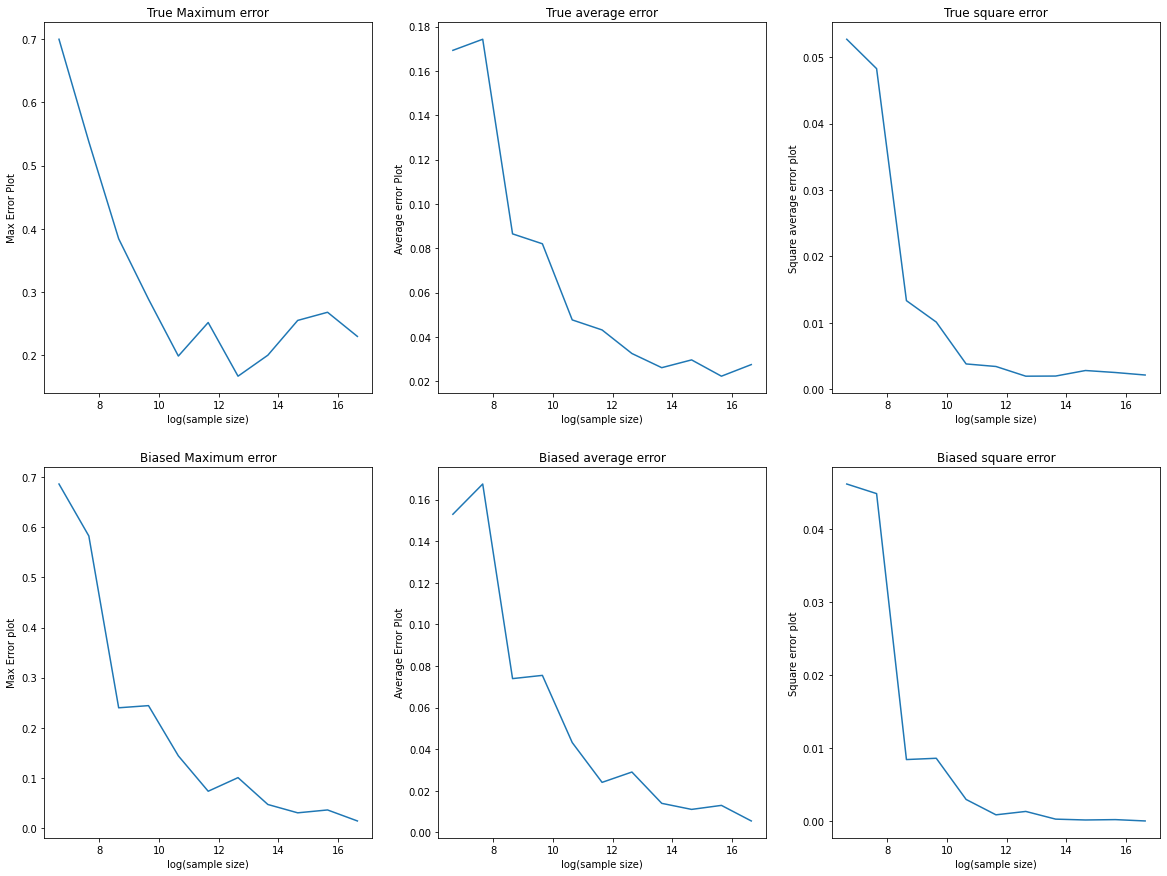
\includegraphics[width=0.95\textwidth]{gaussian_f_3_20_sim_better_bias_estimate.png}
    \caption{Error decay with sample size. The kernel is Gaussian $k(x,y)=\exp(-(\frac{x-y}{h})^2)$. The bandwith is set to $h=0.11$, the noise is set to $\sigma^2=1$, and the function to be estimated is $f(x)=2+x-e^{-x^2}$.
    The experiment is repeated 20 times and the average error curves are plotted.
    }
    \label{fig:error_decay}
\end{figure}


\subsection{ Estimating functions }

\begin{figure}
    \centering
    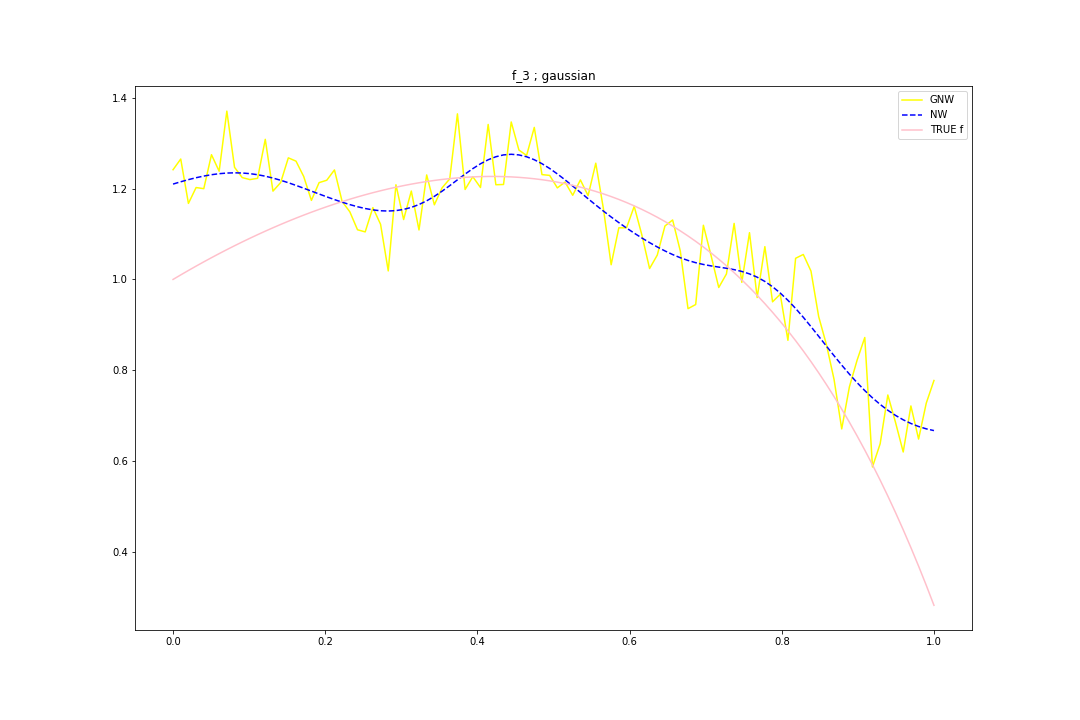
\includegraphics[width=0.5\textwidth]{SSLAN_f_3_gaussian.png}
    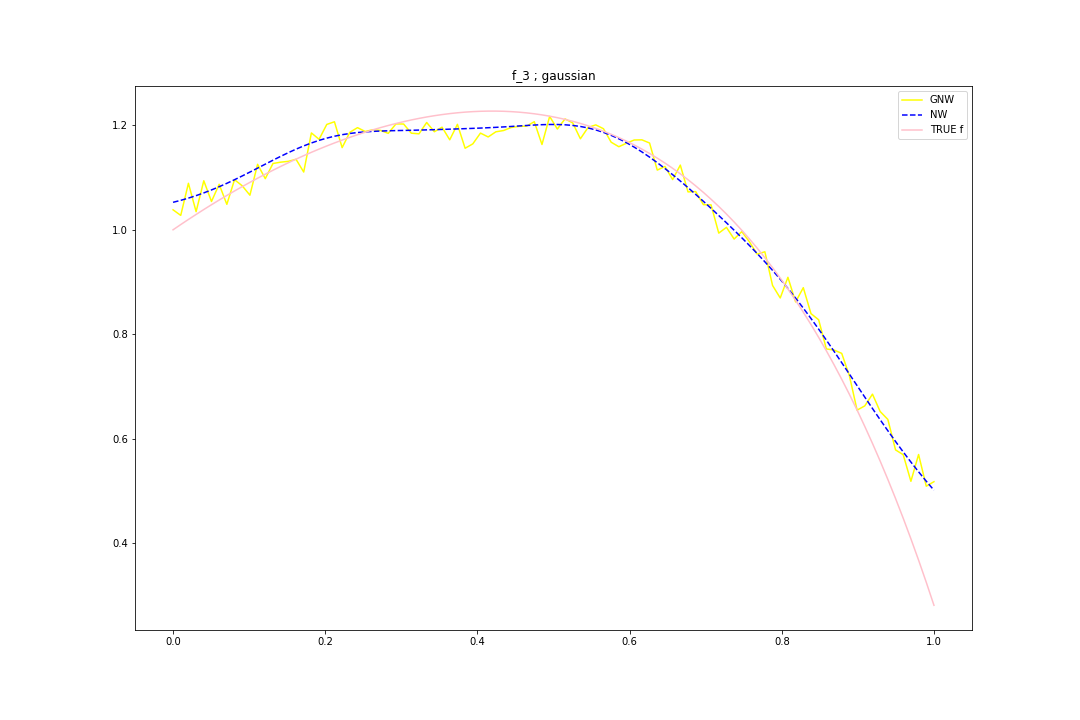
\includegraphics[width=0.5\textwidth]{MSMN_f_3_gaussian.png}
    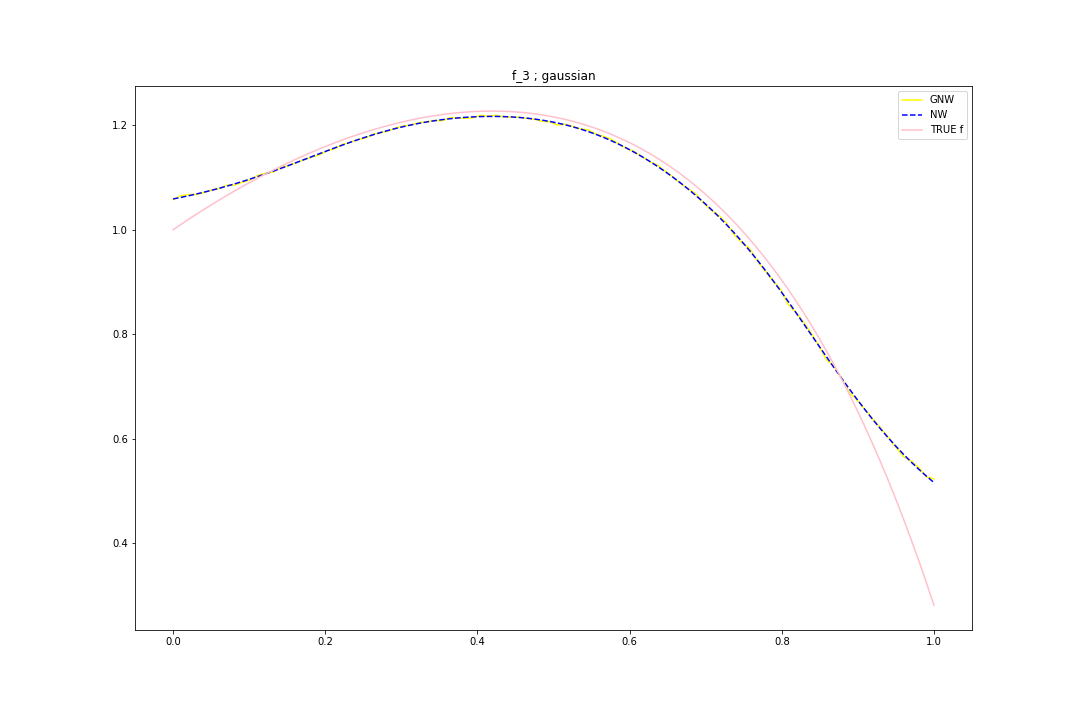
\includegraphics[width=0.5\textwidth]{LSLN_f_3_gaussian.png}
    \caption{Caption}
    \label{fig:my_label}
\end{figure}


\section{Appendix}

\subsection{related work/future plans}

\subsection{Probabilistic proof of the Bernoulli inequality}

The Bernoulli inequality\footnote{In fact the Bernoulli inequality states that for all $y>-1$ and $n\in\mathbb{N}$, $(1+y)^n\geq 1+ny$ but we are only interested in the case $-1<y<0$} states that for all $0<p<1$ and $n\in\mathbb{N}$, 
\begin{equation}
\label{bern_ineq}
    (1-p)^n\geq 1-np
\end{equation}
More generally, for $0<p<1$ and $n\in\mathbb{N}$ we are going to derive bounds for

\begin{equation}
\label{bin_remainder}
b_j=(-1)^j[(1-p)^n-\sum_{l=0}^{j-1}{n \choose l}(-1)^lp^l]
\end{equation}
The proof of Bernoulli's inequality follows easily from the 
observation that $R_1\leq 1$. Indeed, by Lemma \ref{lemma_exp}
\begin{equation*}
    \frac{1-(1-c(x))^n}{nc(x)}=ER_1\leq 1
\end{equation*}
Setting $p=c(x)$ one easily derives inequality (\ref{bern_ineq}). The following lemma provides bounds on 
(\ref{bin_remainder}).
\begin{lemma} For $j=1,2,...,n-1$
\begin{equation*}
    ER_{[j+1]}=\frac{1-jER_{[j]}}{(n-j)c(x)}
\end{equation*}

\end{lemma}
\begin{proof}
Using Equation (\ref{eqn_R}) for $l=j+1,...n$, we have

\begin{equation*}
    a(x,X_l)R_{[j]}=a(x,X_l)R_{[j]\cup\{l\}}
\end{equation*}
Summing these equations for $l=j+1,...,n$ we get

\begin{equation*}
\begin{split}
    1-jR_{[j]}&=1-\frac{j}{j+\sum_{l=j+1}^na(x,X_l)}\\
    &=\frac{\sum_{l=j+1}^n a(x,X_l)}{j+\sum_{l=j+1}a(x,X_l)}\\
    &=\sum_{l=j+1}^na(x,X_l)R_{[j]\cup\{l\}} 
\end{split}
\end{equation*}
Taking expectation and using the fact that $a(x,X_l)$ and $R_{[j]\cup\{l\}}$ are independent, and the fact that $R_{[j]\cup\{l\}}$ and $R_{[j+1]}$ are identically distributed, we get

\begin{equation*}
\begin{split}
    1-jER_{[j]}&=\sum_{l=j+1}^n Ea(x,X_l)R_{[j]\cup\{l\}}\\
    &=\sum_{l=j+1}^nEa(x,X_l)ER_{[j]\cup\{l\}}\\
    &=(n-j)c(x)ER_{[j+1]}
\end{split}    
\end{equation*}
\end{proof}

\begin{corollary}
For $j=1,2,3,...,n-1$ let $b_j$ be given by (\ref{bin_remainder}). Then 

\begin{equation*}
    \frac{j}{n}{n \choose j}p^j<b_j<{n\choose j}p^j
\end{equation*}
\end{corollary}

\begin{proof}
Consider the sequence $b^{'}_j=\frac{b_j}{j{n\choose j}p^j}$. It is easy to verify that $b^{'}_1=ER_1$ and that 

\begin{equation*}
    b^{'}_{j+1}=\frac{1}{1}
\end{equation*}
\end{proof}



\subsection{A Generalization: Higher order GNW estimators}

In this section we discuss a generalization of the Graphical Nadaraya Watson which averages the observations $Y_i$ over vertices which have fixed graph distance $m$ from $X$. Using Corollary 1 we show that this estimator concentrates around the quantity $\frac{T_k^m(f)(X)}{c_m(X)}$ with probability 

\subsubsection{Second order GNW estimator \texorpdfstring{$\hat{f}_{GNW,m}$}{Lg}}

The proposed estimator $\hat{f}_{GNW}$ does not take advantage of the graph structure of the data. The estimator at a vertex
$v$ is based only on neighbours of 
$v$. In order to account for the potential influence of vertices which are not direct neighbours of $v$, we introduce the weights\footnote{ At this point we have not stated anything about self edges in the observed graph. As long as the variables $a(X_i,X_i)$ are
bounded and 
independent, their contribution will vanish for large n so to simplify the exposition we assume that $a(X_i,X_i)=0$.
}
\paragraph{Remark 8 (Higher order GNW Estimators)}
Given $1\leq m\leq n$, we introduce the weights

\begin{equation*}
    w_m(X_i,X)=\sum_{J_{i}} \prod_{j=0}^{m-1} a(X_{i_j},X_{i_{j+1}})
\end{equation*}
Here, $J_{i}=(i,i_1,...,i_{m-1})$ is a $m$-tuple of distinct indicies with the convention that
$i_0=i$ and $X_{i_m}$ is identified with $X$ and the sum is taken over all such $m$-tuples $J_i$. We introduce the \textbf{GNW estimator of order m}:
\begin{equation*}
    \hat{f}_{GNW,m}(X)=\frac{\sum_{i=1}^n Y_iw_m(X_i,X)}{\sum_{i=1}^n w_m(X_i,X)}
\end{equation*}
The case $m=2$ which was discussed in the previous paragraph is can be used as an inductive step in proving a concentration inequality for $\hat{f}_{GNW,m}$. It can be shown in a simmilar manner in which Lemma 6 was shown that 
As $pdx$ is a probability measure, compositions of $T_k$ of any order
$m\geq 1$
are well defined, and 

\begin{equation*}
    T_k^m(f)(x)=\int_{\mathbb{R}^d} T_k^{m-1}(f(z))k(x,z)p(z)dz
\end{equation*}




\begin{equation*}
P(|\frac{(n-m)!}{n!}\sum_{i=1}^n f(X_i)w_m(X_i,X)-\frac{(n-(m-1))!}{n!}\sum_{i=1}^n T_k(f)(X_i)w_{m-1}(X_i,X)|\geq \delta)\leq 2n^{m-1}\exp(-\frac{2\delta^2(n-(m))}{5B})
\end{equation*}
\paragraph{Remark 9 (Application to the Stochastic Block Model)}
More formally, $SBM(n,p,W)$ where $n$ is a positive integer, $p=(p_1,...,p_K)$ is $K$ dimensional vector with $0\leq p_l\leq 1$ and $\sum_{l=1}^Kp_l=1$ and $W$ is a $K\times K$ symmetric matrix with entries $0\leq w_{i,j}\leq 1$ generates edges on vertices $[n]$ by first randomly assigning a community $C_1,...,C_K$ to each node with $P(i\in C_l)=p_l$ (these assignments are independent over distinct vertices) and then generating edges depending on the community of the endpoints of the edge, that is $P(i\sim j| i\in C_l,j\in C_s)=w_{ls}$. There are several questions in the $SBM$ model such as deciding if an observed graph is indeed sampled by an $SBM$, under which conditions is there a way to fully or partially recover communities based on a single observed graph. The Stochastic Block Model has a long history in the statistics literature (  \cite{Snijders}). For recent developments we refer to (\cite{Abbe}).



The stochastic block model $SBM(n,W,p)$ (where $n$ is a positive integer, $W$ a $k\times k$ symmetric matrix with entries in $[0,1]$ and
$p=(p_1,...,p_k)$ is such that
$p_1+...+p_k=1$ and $p_i>0$, $i=1,...,n$)
is a random graph model that can be defined as follows:
Each node $i$ belongs to one of $k$
(disjoint) sets $B_1,...,B_k$ independently from the other nodes $j\neq i$ and with $P(i\in B_l)=p_k$, 
$1\leq l \leq k$. Then for any two blocks $B_l, B_s$,  we have

\begin{equation*}
    P(i\sim j|i\in B_l,j\in B_s)=W_{l,s}
\end{equation*}
The nodes $1,2,....,n$ may be thought of as individuals, the sets $B_l$ may be thought of as different blocks or communities and the parameters $W_{l,s}$ as the probability of connection between blocks $B_l$ and $B_s$. The Stochastic block model is a special case of Latent position model. Indeed, 
p to be a uniform $[0,1]$ distribution with kernel 

\begin{equation*}
    k(x_{i},x_{j})=\sum_{l\leq s} W_{l,s} I(x_{i}\in B_l, x_{j}\in B_s)
\end{equation*}

where $B_l$ is the semi-open interval with endpoints $\sum_{j=1}^{l-1}p_j$ and $\sum_{j=1}^{l}p_j$.
Then it is easy to see that the probability of edge between two vertices $i,j$ 
in this Latent position model is equal to the probability of edge between the vertices $i,j$ in a Stochastic block model $SBM(n,W,p)$. From here 
and the previous remark 
it follows that edge related statistics such as $w_m(i,j)$ can identyify the individuals in blocks with high probability, under suitable  assumptions that these statistics differ among blocks. We omit the details.



\printbibliography
\nocite{*}






\end{document}
